%!TEX root = _thesis.tex
\chapter{実験結果と考察}

\section{ジェスチャ識別結果}

各ジェスチャを行なっている時のセンサデータをラベル付けし,
SVMモデルを5-fold cross validationを行なった結果を以下のFig.\ref{fig:matrix}に示す.

\begin{figure}[H]
  \centering
  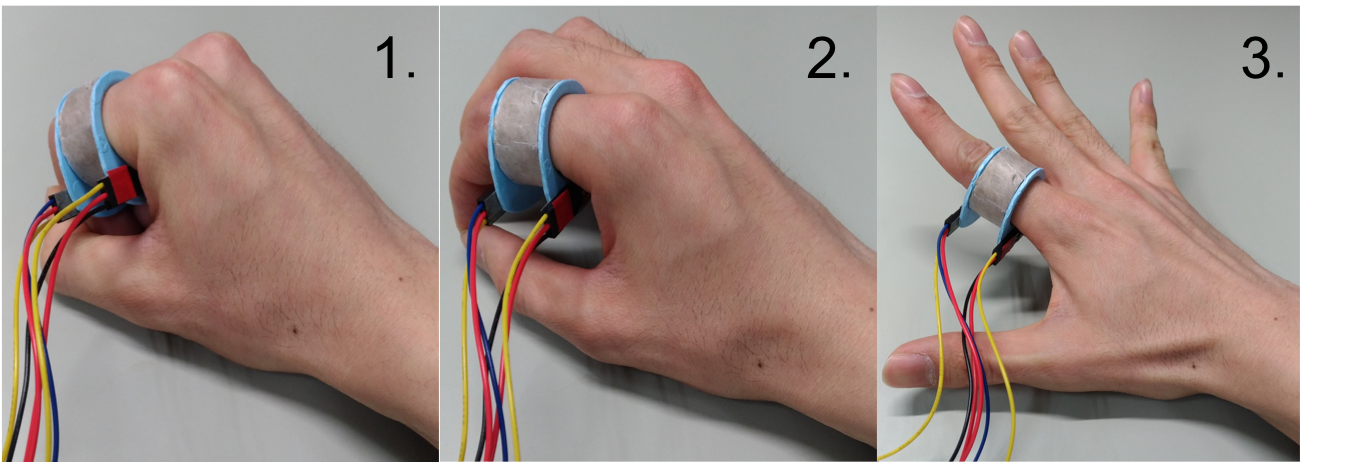
\includegraphics[width=0.8\linewidth]{fig/gesture}
  \caption{Prepared hand-gesture set}
  \label{fig:gesture}
\end{figure}

\begin{figure}[H]
  \centering
  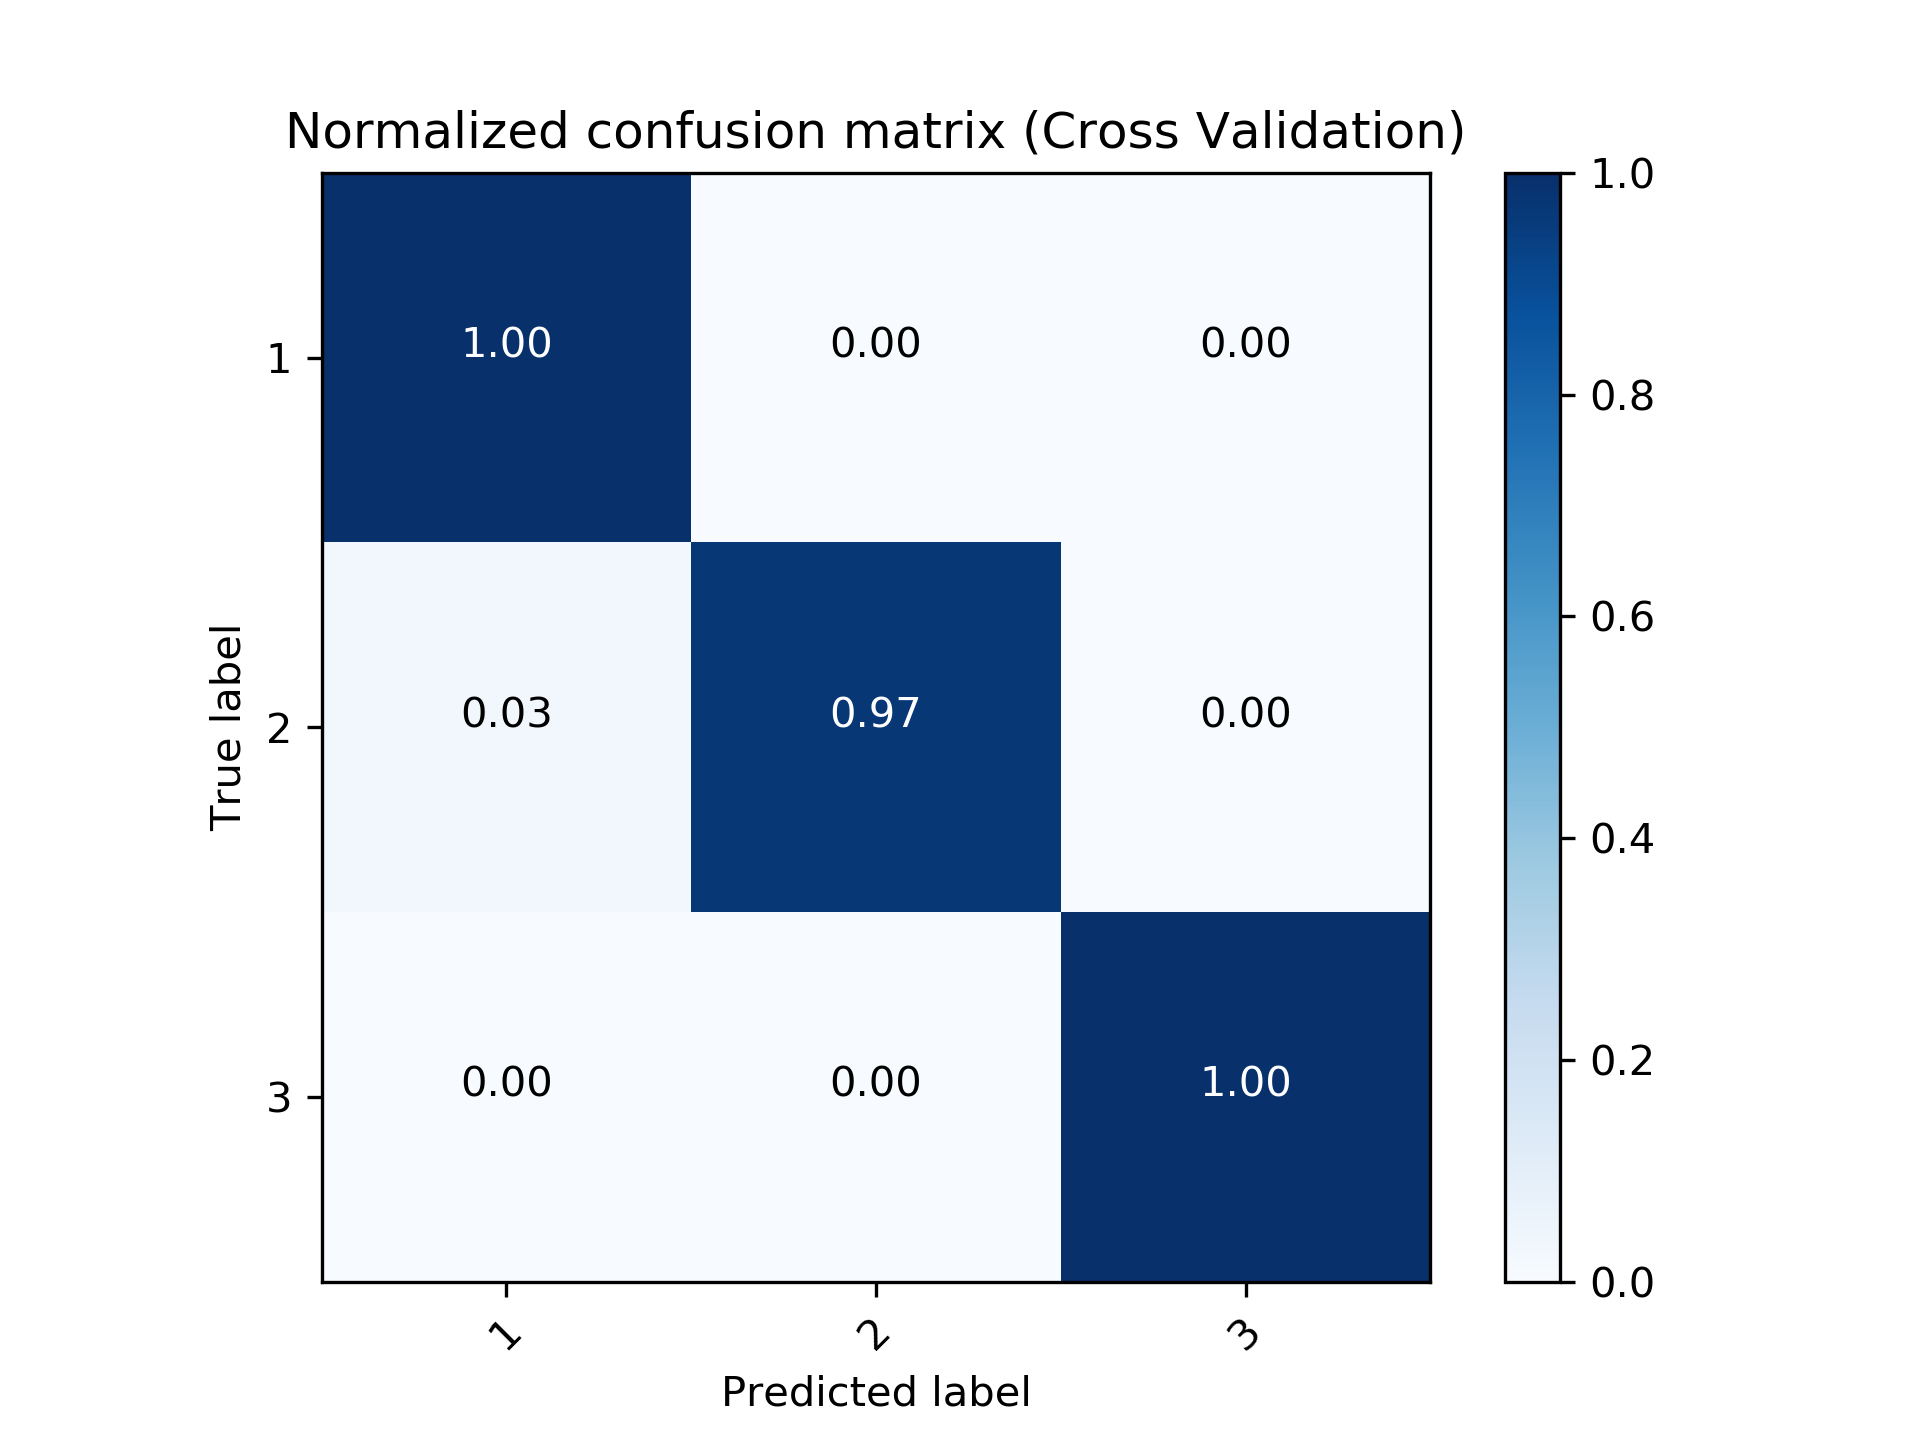
\includegraphics[width=0.8\linewidth]{fig/confusion_matrix}
  \caption{Confusion matrix of 3-gesture}
  \label{fig:matrix}
\end{figure}


Fig.\ref{fig:matrix}より,ジェスチャ1と3を100\%の正解率で識別することが可能であることが分かった.
五分割交差検証を行った結果,ジェスチャ全体の平均正解率は98.9\%,分散3.9\%であった.この結果から本手法により三つのジェスチャの識別が可能であることが示された.

\section{関節角度推定結果}


以下に実験結果を示す.以下の表は被験者ごとの,推定角度と正解角度のMean Absolute Errorと相関係数を示した表である.


\begin{table}[H]
  \caption{MAE and R between{}
True Angle and Predicted Angle (n=10)}
  \label{table:data_type}
  \centering
  \begin{tabular}{ccc}
    \hline
    Subjects  & Mean Absolute Error$^\circ$  & Correlation coefficient  \\
    \hline \hline
    A  & 2.71 & 0.993\\
    B  & 2.62 & 0.995\\
    C  & 6.61 & 0.985\\
    D  & 5.01 & 0.994\\
    E  & 2.33 & 0.995\\ 
    F  & 2.87 & 0.995\\
    G  & 1.57 & 0.998\\
    H  & 2.87 & 0.992\\
    I  & 3.04 & 0.986\\
    J  & 2.41 & 0.994\\
    \hline
  \end{tabular}
\end{table}

MAEの被験者平均は $3.20^\circ$ (SD=$1.48^\circ$)であった.
また,Rの被験者平均は0.991(SD=0.005)であった.
Manumeterでは指の関節角度の推定精度MAEが$4.7^\circ$である\cite{Friedman2014}.
よって, 本手法は既存の手法よりも高い関節角度の推定精度を持つことが言える.

以下のFig.\ref{fig:linear}は,被験者ごとに推定角度に基づいて,正解角度を線形回帰により求めた図である.0,90度の時のプロットの分散が小さいことが分かる.これは,キャリブレーションを0,90度の際のジェスチャを基準として行なっているためだと考えられる.(c)ではLinear Regressionの傾きが,(d)では切片が,Unityから外れているが,その他は,大きく予測を外しているプロットもなく,良好な角度推定ができていると言える.

\begin{figure}[H]
\begin{center}
\begin{tabular}{cc}
\subfigure[Subject A]{
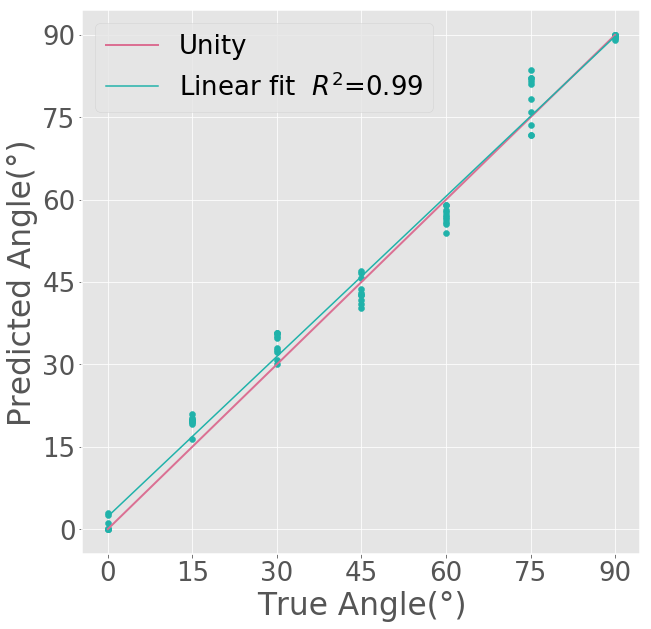
\includegraphics[scale=0.3]{fig/sub1.png}
} &
\subfigure[Subject B]{
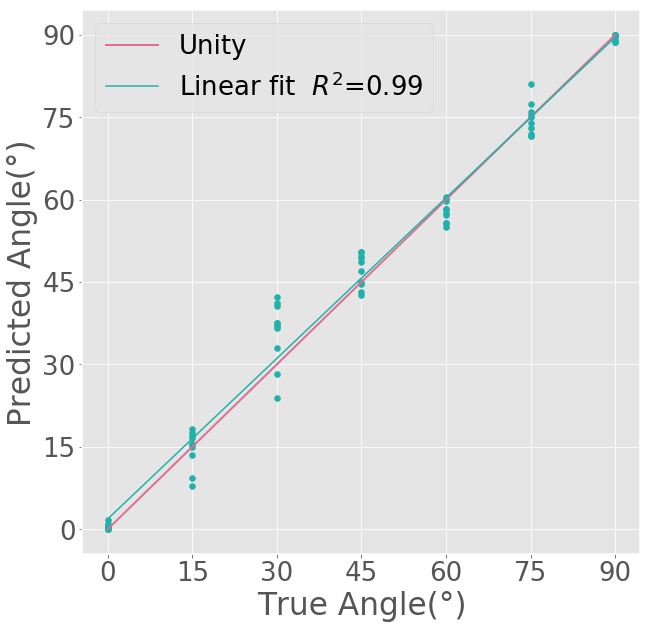
\includegraphics[scale=0.3]{fig/sub2.png}
} \\
\subfigure[Subject C]{
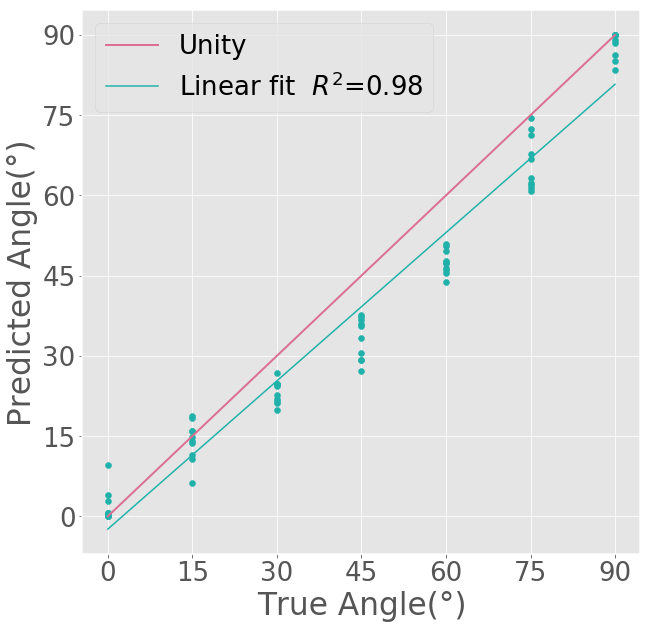
\includegraphics[scale=0.3]{fig/sub3.png}
} &
\subfigure[Subject D]{
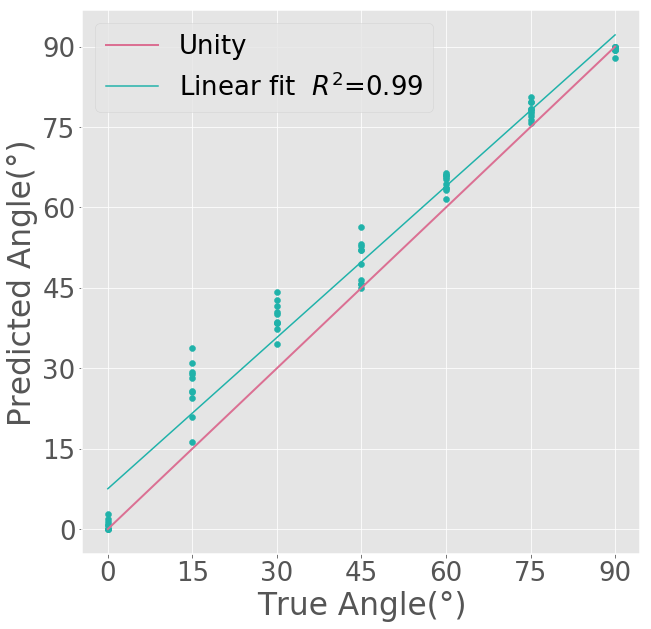
\includegraphics[scale=0.3]{fig/sub4.png}
} \\
\subfigure[Subject E]{
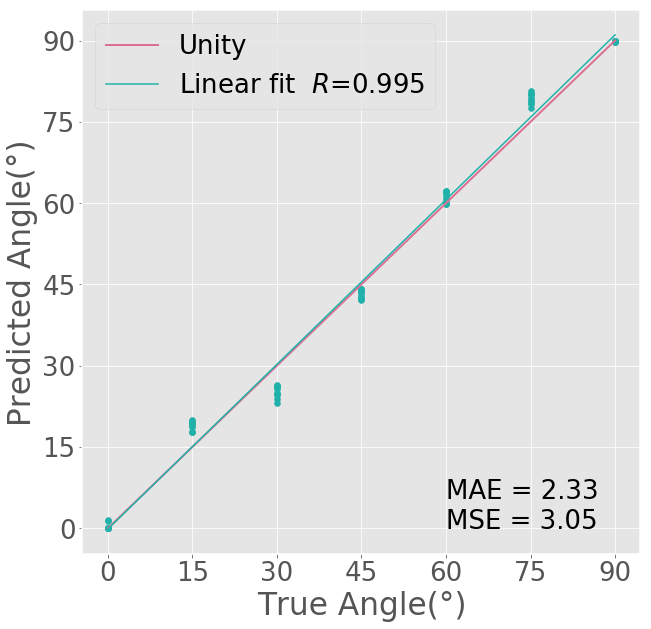
\includegraphics[scale=0.3]{fig/sub5.png}
} &
\subfigure[Subject F]{
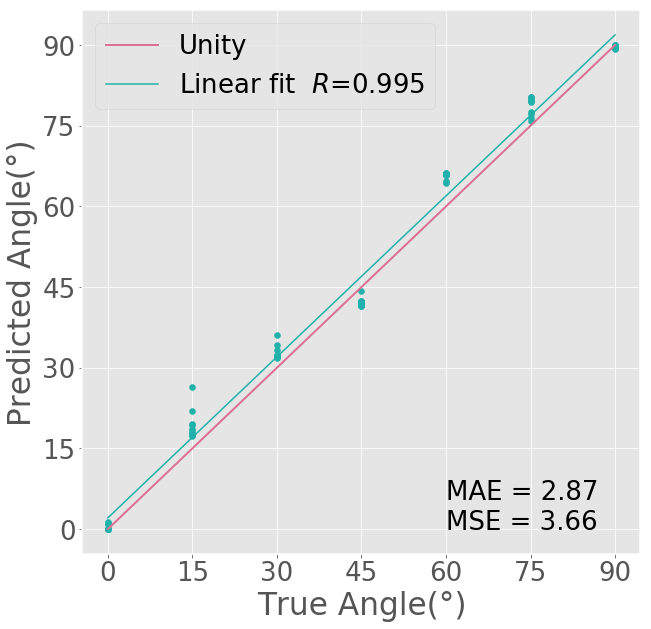
\includegraphics[scale=0.3]{fig/sub6.png}
} \\
\end{tabular}
\end{center}
\end{figure}


\begin{figure}[H]
\begin{center}
\begin{tabular}{cc}
\setcounter{subfigure}{6}
\subfigure[Subject G]{
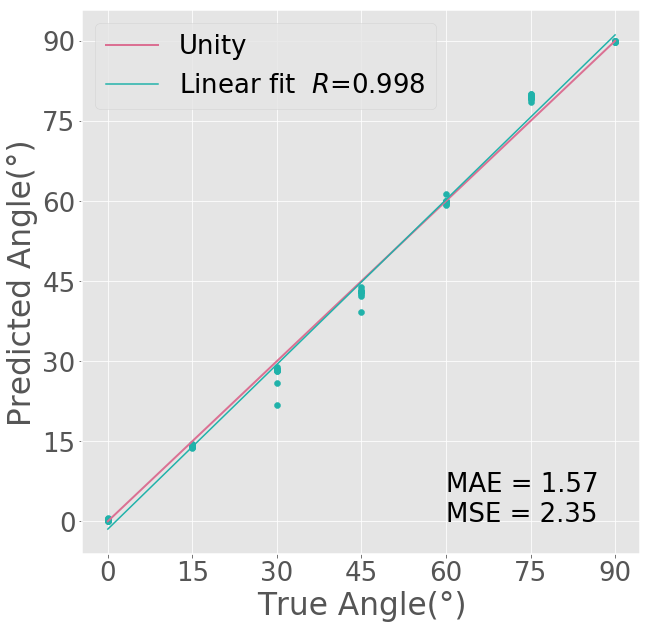
\includegraphics[scale=0.3]{fig/sub7.png}
} &
\subfigure[Subject H]{
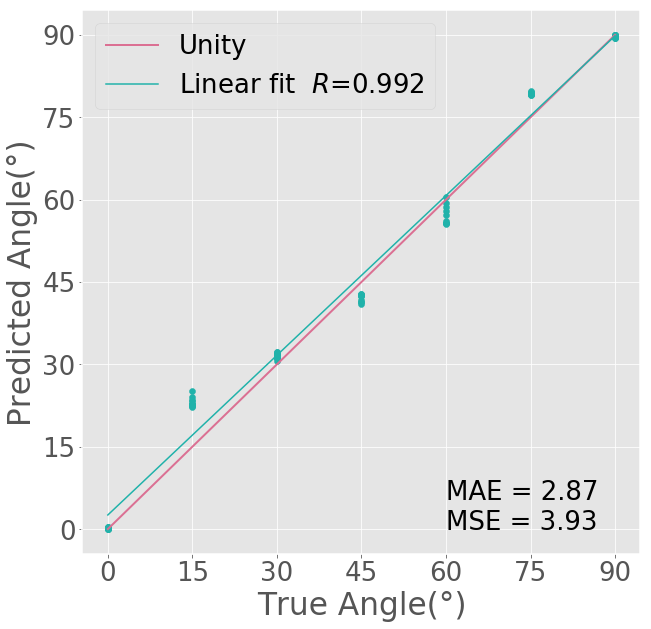
\includegraphics[scale=0.3]{fig/sub8.png}
} \\
\subfigure[Subject I]{
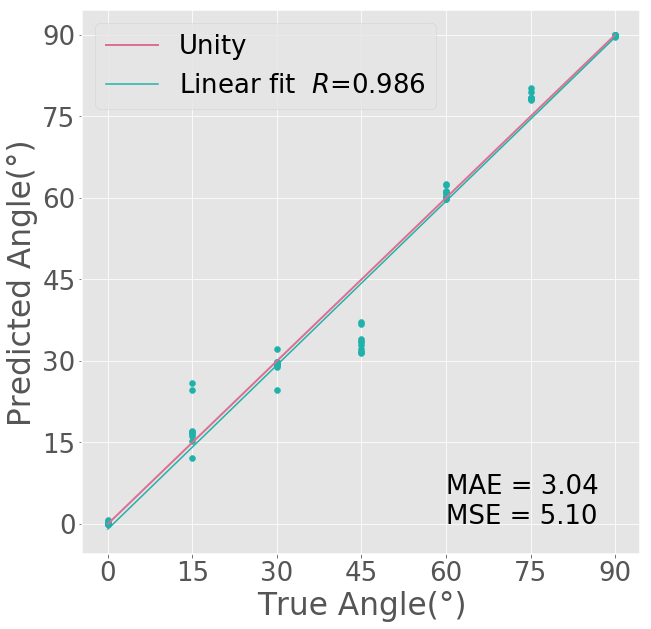
\includegraphics[scale=0.3]{fig/sub9.png}
} &
\subfigure[Subject J]{
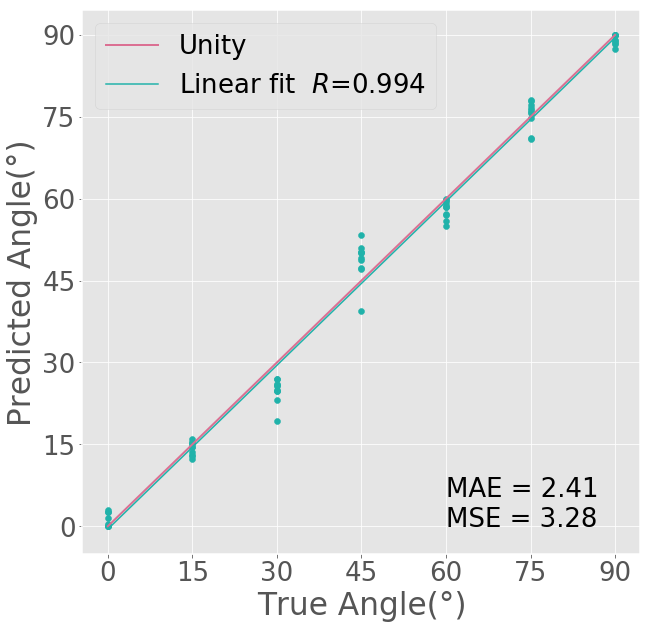
\includegraphics[scale=0.3]{fig/sub10.png}
} \\
\end{tabular}
\caption{Observed-Predicted Plot}
\label{fig:linear}
\end{center}
\end{figure}


以下のFig.\ref{fig:res}は,被験者ごとに,正解角度と予測角度の誤差$Res_i$をプロットしたグラフである.


\begin{figure}[H]
\begin{center}
\begin{tabular}{cc}
\subfigure[Subject A]{
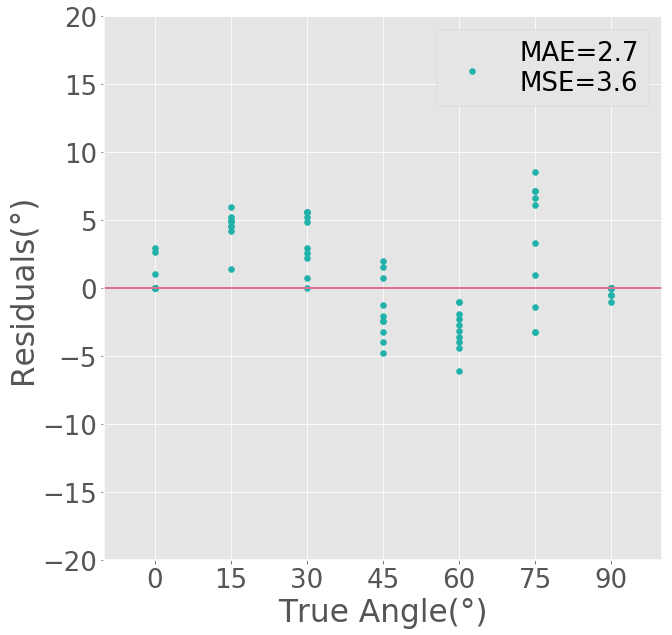
\includegraphics[scale=0.3]{fig/sub1r.png}
} &
\subfigure[Subject B]{
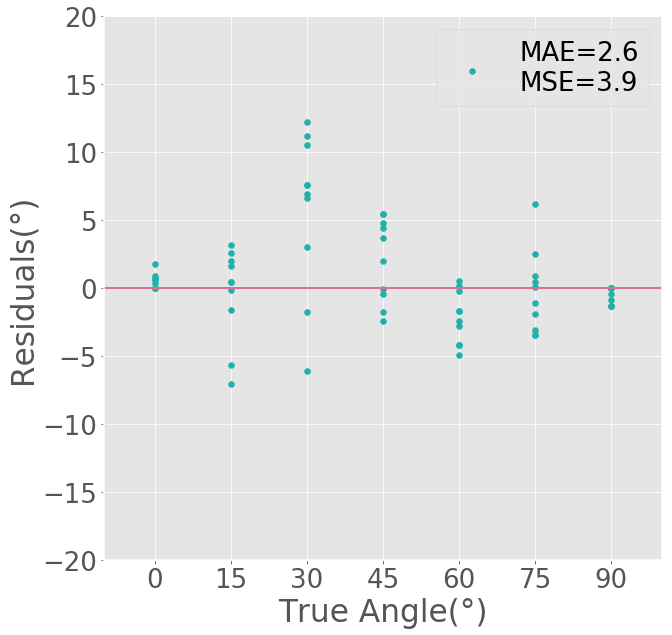
\includegraphics[scale=0.3]{fig/sub2r.png}
} \\
\subfigure[Subject C]{
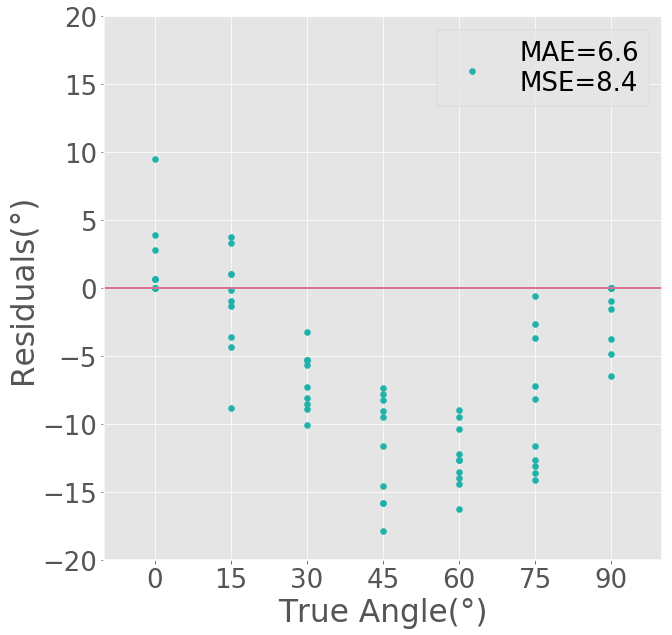
\includegraphics[scale=0.3]{fig/sub3r.png}
} &
\subfigure[Subject D]{
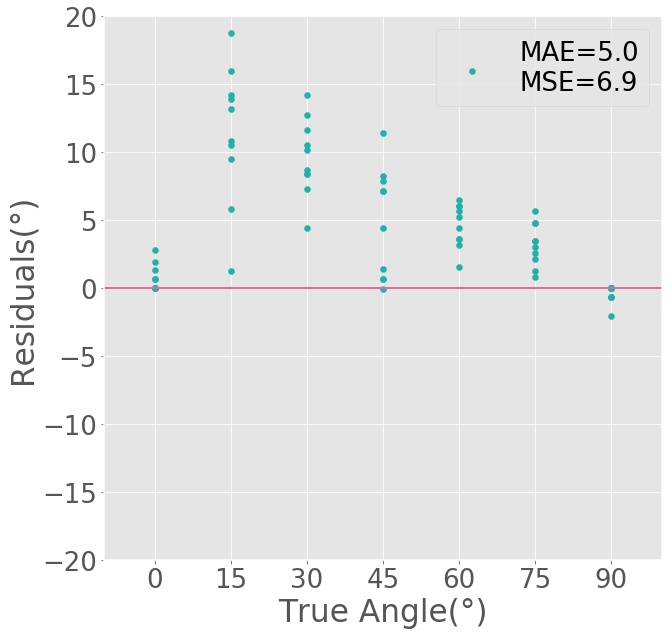
\includegraphics[scale=0.3]{fig/sub4r.png}
} \\
\subfigure[Subject E]{
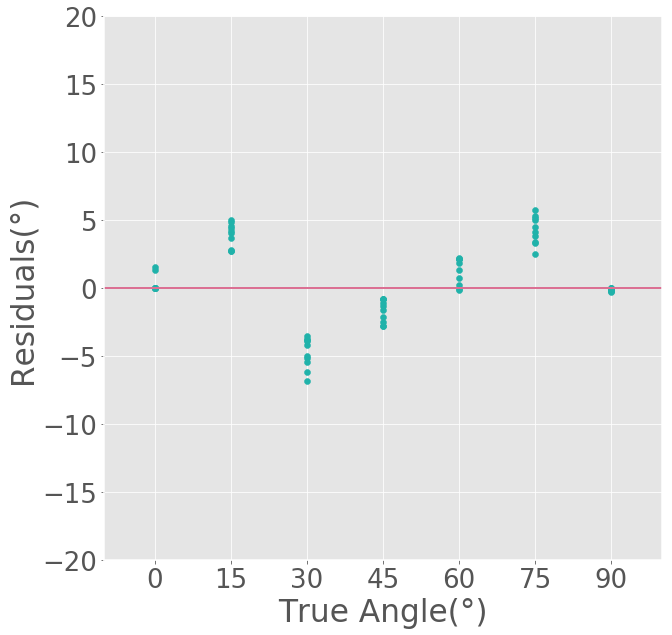
\includegraphics[scale=0.3]{fig/sub5r.png}
} &
\subfigure[Subject F]{
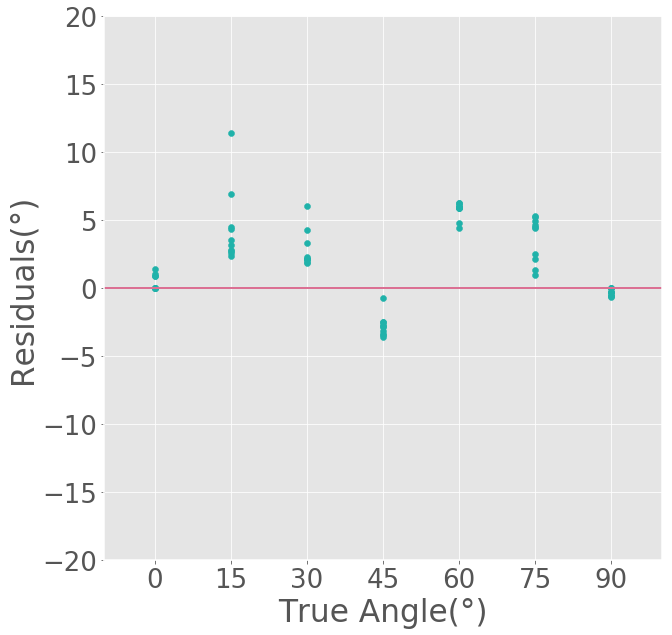
\includegraphics[scale=0.3]{fig/sub6r.png}
} \\
\end{tabular}
\end{center}
\end{figure}


\begin{figure}[H]
\begin{center}
\begin{tabular}{cc}
\setcounter{subfigure}{6}
\subfigure[Subject G]{
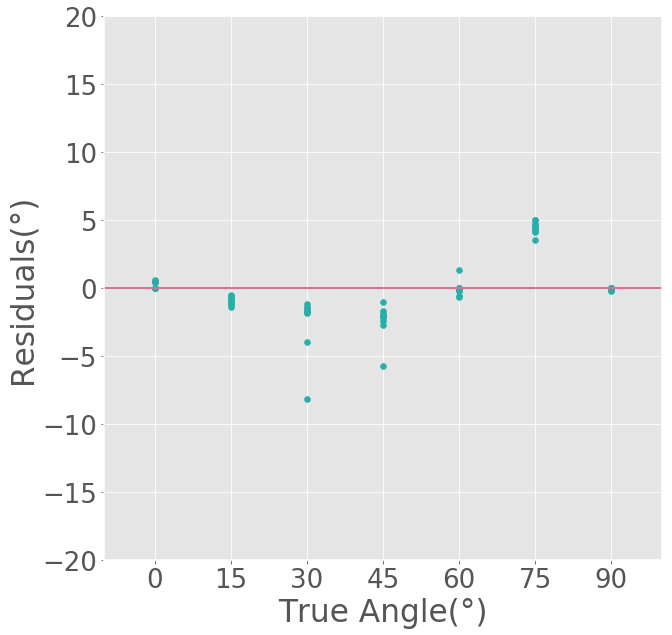
\includegraphics[scale=0.3]{fig/sub7r.png}
} &
\subfigure[Subject H]{
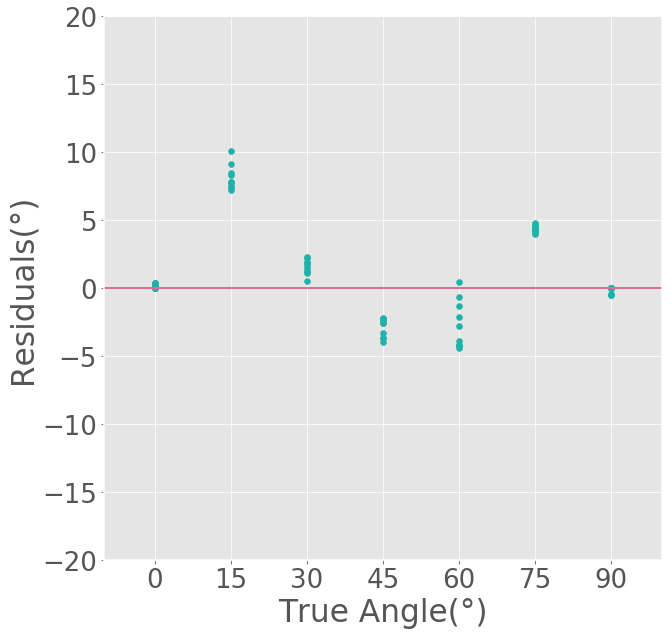
\includegraphics[scale=0.3]{fig/sub8r.png}
} \\
\subfigure[Subject I]{
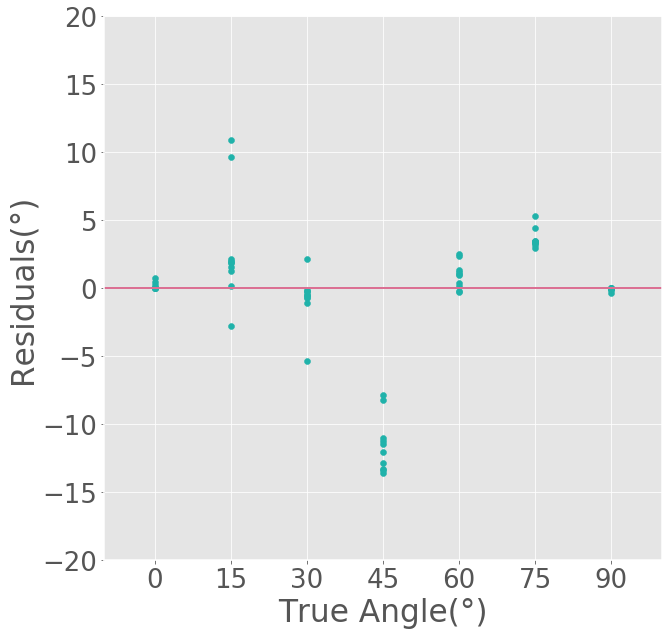
\includegraphics[scale=0.3]{fig/sub9r.png}
} &
\subfigure[Subject J]{
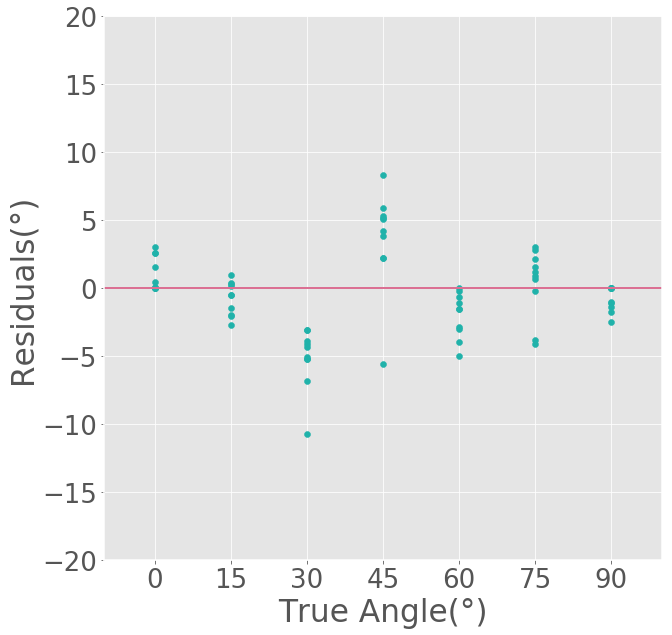
\includegraphics[scale=0.3]{fig/sub10r.png}
} \\
\end{tabular}
\caption{Residuals plot}
\label{fig:res}
\end{center}
\end{figure}


結果から本手法により関節角度が推定でき,手指使用量を計測可能であることが示唆された.


\section{Acceleromertyとの日常生活,リハビリ動作評価の比較}

得られたデータは,正規性,等分散性が認められなかったため,分散分析としてフリードマン検定を行なった.
この時サンプルサイズはn=8である.
フリードマン検定を行なった結果,代表値に差が見られた.フリードマン検定の結果を以下の\ref{table:friedman}に示す.

\begin{table}[H]
  \caption{Friedman test}
  \label{table:friedman}
  \centering
  \begin{tabular}{rll}
    \hline 
measure &  p-value  & $\eta^2$\\
    \hline \hline
Angle     & 2.214751e-07****&0.5945477\\
Acceleration  & 2.039236e-08****&0.6398353\\

    \hline
  \end{tabular}
\end{table}

Angle,Accelerationともに,タスク間で代表値に違いがあったため,
Games-Howel法で各タスクの1対1の対比較を行なった.
Games-Howel法は,正規性,等分散性の制限のないノンパラメトリック検定である.
Games-Howel法で検定した結果を以下のTable.\ref{table:games}に示す.
eat vs. fold,eat vs. peg,fold vs. write,peg vs. writeの比較ではAngle,Accelerationともに有意差が見られた.
eat vs. wipe,eat vs. write,fold vs. type,peg vs. typeの比較ではAccelerationのみに有意差が見られた.
fold vs. wipe ,peg vs. wipeの比較ではAngleのみに有意差が見られた.

\begin{table}[H]
  \caption{Games-Howel test p-value}
  \label{table:games}
  \centering
  \begin{tabular}{rll}
    \hline 
Paired comparison &  Angle p-value  & Acceleration p-value\\
    \hline \hline
eat vs. fold     & 0.02096*&0.00028***\\
eat vs. peg      & 0.00249**&0.00001***\\
eat vs. type     & 0.30367&0.09258\\
eat vs. wipe     & 0.99997&0.03925*\\
eat vs. write    & 0.61927&0.02215*\\
fold vs. peg     & 0.95225&0.70476\\
fold vs. type    & 0.16702&0.01238*\\
fold vs. wipe    & 0.02079*&0.42099\\
fold vs. write   & 0.03235*&0.00105**\\
peg vs. type     & 0.17113&0.04332*\\
peg vs. wipe     & 0.00164**&0.87725\\
peg vs. write    & 0.00380**&0.00011***\\
type vs. wipe    & 0.39653&0.74382\\
type vs. write   & 0.63400&0.80855\\
wipe vs. write   & 0.93563&0.22543\\
    \hline
  \end{tabular}
\end{table}


被験者8人の各タスクごとの関節角度の変化量の合計を以下のボックスプロットFig.\ref{fig:angle_usage}に示す.


\begin{figure}[H]
  \centering
  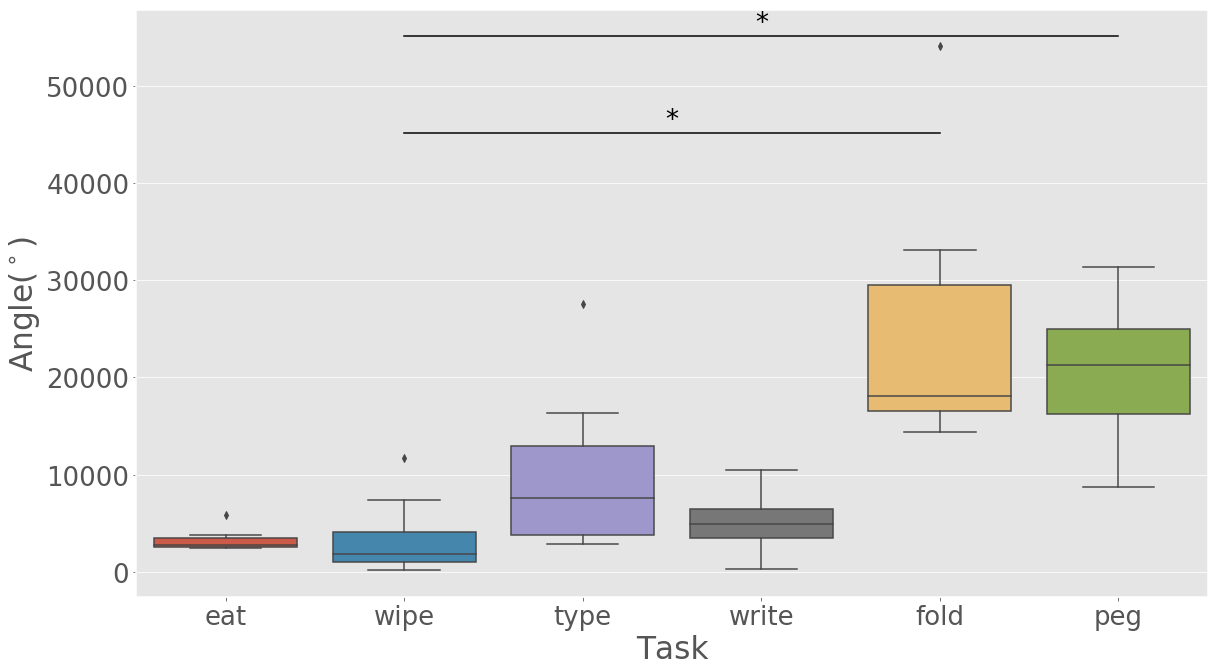
\includegraphics[width=0.8\linewidth]{fig/boxplot_angle}
  \caption{Aggrigated usage of finger }
  \label{fig:angle_usage}
\end{figure}


被験者8人の各タスクごとの加速度の変化量の合計を以下のボックスプロットFig.\ref{fig:accel_usage}に示す.

\begin{figure}[H]
  \centering
  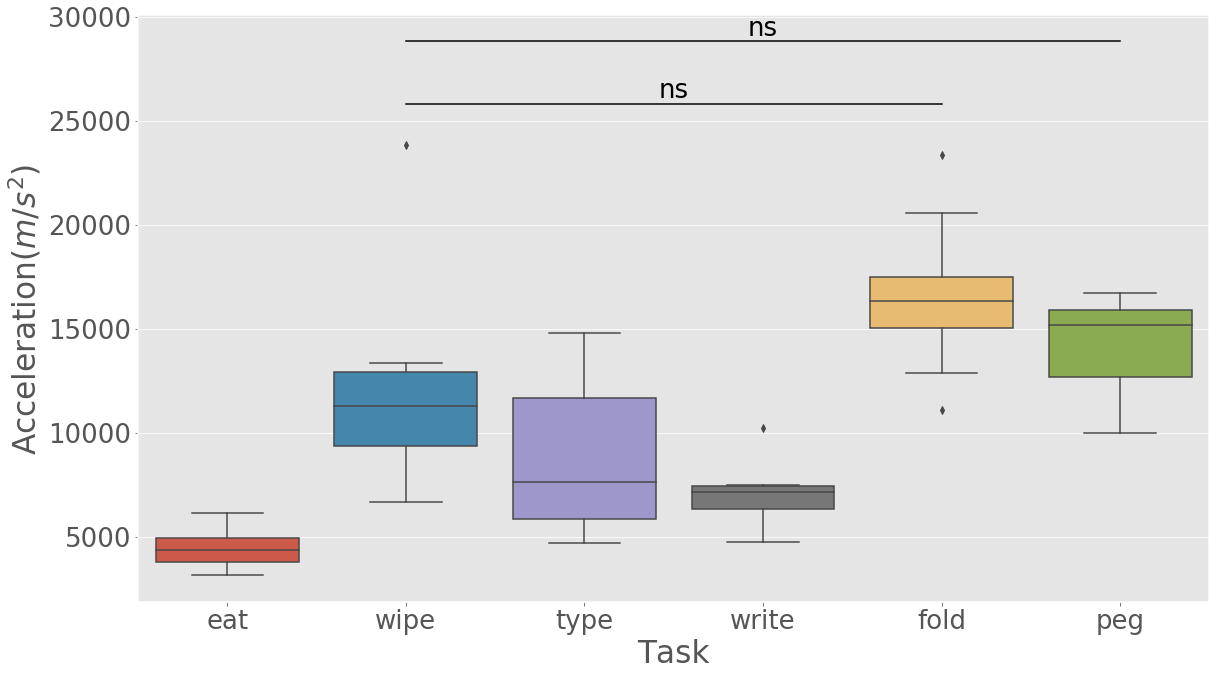
\includegraphics[width=0.8\linewidth]{fig/boxplot_accel}
  \caption{Aggrigated usage of arm}
  \label{fig:accel_usage}
\end{figure}

fold vs. wipeとpeg vs. wipe 比較のとき,
Angleには有意差が認められ,Accelerationには有意差が認められなかった.
なお,Fig.\ref{fig:angle_usage}とFig.\ref{fig:accel_usage}には,それらの注釈を記述した.



\section{考察}
Accelerometryと本手法を組み合わせることで,腕の使用量のみではなく,指の使用量の評価が行えることが示唆された.

\begin{table}[H]
  \caption{Comparison of our proposed device and other device}
  \label{table:comparison}
  \centering
  \begin{tabular}{ccccc}
    \hline
    System &  Accelerometry with Proposed device & Accelerometry & Data glove & Motion Capture System\\
    \hline \hline
    a&A&A&A&A\\


    \hline
  \end{tabular}
\end{table}




